\documentclass[12pt,a4paper]{article}

% package importing
%\usepackage[margin=2cm]{geometry}
\usepackage{geometry}
 \geometry{
 a4paper,
 %total={170mm,257mm},
 left=10mm,
 top=20mm,
 right=10mm,
 bottom=20mm,
 }
 		%$$$$$$ fonts settings $$$$$$%
%\usepackage[sc]{mathpazo}  %for palatino font
%\usepackage{eulervm}  %for Euler maths font

		%$$$$$$ package imports $$$$$$%
\usepackage{amsmath}  %for mathematics
\usepackage{titlesec}  %for title spacing only
\usepackage{lipsum}  %random huge text generation
\usepackage{titlesec} %for changing font of titles 
\usepackage{amssymb}  %for real number set symbol
\usepackage{amsthm}  %for mathematics package
\usepackage{mathtools}  %for floor and ceiling
\usepackage{algorithmicx}  %for dynamic algorithm
\usepackage{algorithm}  %algorithm micro
\usepackage{algpseudocode}  %pseudocode commands
\usepackage{wrapfig}  %for wrapping figures around text
\usepackage{multicol}  %for multiple columns floats
\usepackage{enumitem}  %for enumerate numbering
\usepackage{url}   %for writing the url
\usepackage{color}  %for colorred text
\usepackage{tcolorbox}  %for colour box highlighting
\usepackage{listings}  %for code listing

% $$$$$$$$$ new command and theorems self-defined
\theoremstyle{definition}
\newtheorem{theorem}{Theorem}[section]
\newtheorem{corollary}{Corollary}[theorem]
\newtheorem{lemma}[theorem]{Lemma}
\newtheorem*{remark}{Remark}
\newtheorem{definition}{Definition}[section]
\newtheorem{example}{Example}[section]
\newtheorem{notation}{Notation}[section]
\newtheorem{algoalgorithm}{Algorithm}[section]

% $$$$$$$$ set general info $$$$$$$
\title{\textsl{National University of Singapore} \\ \textbf{CS2106 Operating System}\\ Midterm Summary Notes}
\author{\textit{Dong Shaocong} A0148008J}

% $$$$$$$$ package parameter setting $$$$$$$$$

% for title spacing {left}{before}{after}  ----------------------------
\titlespacing\section{0.5pt}{10pt plus 2pt minus 2pt}{2pt plus 2pt minus 1pt}
\titlespacing\subsection{0.5pt}{10pt plus 2pt minus 2pt}{2pt plus 2pt minus 1pt}
\titlespacing\subsubsection{0.5pt}{10pt plus 2pt minus 2pt}{2pt plus 2pt minus 1pt}

% for title font specifications  ------------------------------------------
\titleformat{\section}
  {\normalfont\fontsize{17}{17}\bfseries}
  {\thesection}{1em}{}
  
\titleformat{\subsection}
  {\normalfont\fontsize{15}{15}\bfseries}{\thesection}{1em}{}
  
\titleformat{\subsubsection}
  {\normalfont\fontsize{13}{13}\bfseries}{\thesection}{1em}{}

% declare floor and ceiling functions   ------------------------------------------
\DeclarePairedDelimiter\ceil{\lceil}{\rceil}
\DeclarePairedDelimiter\floor{\lfloor}{\rfloor}

% set the numbering of enumerate to numbers------------------------------------------
\setlist[enumerate]{label*=\arabic*.}
%\setlist{nolistsep}
\newenvironment{myitemize}
{ \begin{itemize}
    \setlength{\itemsep}{5pt}
    \setlength{\parskip}{0pt}
    \setlength{\parsep}{0pt}     }
{ \end{itemize}                  } 
\newenvironment{myenumerate}
{ \begin{enumerate}
    \setlength{\itemsep}{5pt}
    \setlength{\parskip}{0pt}
    \setlength{\parsep}{0pt}     }
{ \end{enumerate}                } 

% $$$$$$$$$ math symbols cheatsheet
% Caligraphic letters: $\mathcal{A}$ 
% Mathbb letters: $\mathbb{A}$
% Mathfrak letters: $\mathfrak{A}$ 
% Math Sans serif letters: $\mathsf{A}$ 
% $$$$$ color text commands ------------
\newcommand{\redtt}[1]{{\color{red}\texttt{#1}}}
\newcommand{\bluett}[1]{{\color{blue}\texttt{#1}}}
\newcommand{\browntt}[1]{{\color{brown}\texttt{#1}}}
\newcommand{\bluebf}[1]{{\color{blue} \huge \textbf{#1}}}
\renewcommand{\emph}[2]{\redtt{#1} \bluebf{#2}}
%-------------------------------------------------------

% $$$$$$$$ start of documents $$$$$$$$$
\begin{document}
\maketitle

\section{Basic Idea}
\begin{definition}{\textbf{Operating System}}
	is a suite (i.e. a collection) of specialised software that:
	\begin{myitemize}
		\item Gives you access to the hardware devices like disk drives, printers, keyboards and monitors.
		\item Controls and allocate system resources like memory and processor time.
		\item Gives you the tools to customise your and tune your system.
	\end{myitemize}
\end{definition}
\begin{example}
	LINUX, OS X (or MAC OS, a variant of UNIX), Windows 8
\end{example}

\begin{tcolorbox}
	\textsf{What are Operating System?} It usually consists of several parts. (\textsf{Onion Model})
	
	\begin{myitemize}
		\item Bootloader – First program run by the system on start-up. Loads remainder of the OS kernel. 
		\begin{myitemize}
			\item On Wintel systems this is found in the Master Boot Record (MBR) on the hard disk.
		\end{myitemize}
		\item Kernel – The part of the OS that runs almost continuously. 
		\item System Programs – Programs provided by the OS to allow:
		\begin{myitemize}
		\item Access to programs.
		\item Configuration of the OS.
		\item System maintenance, etc.
		\end{myitemize}
	\end{myitemize}
		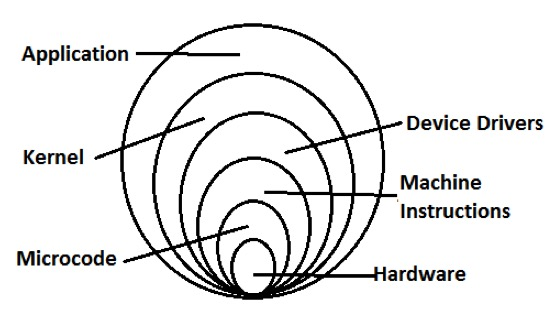
\includegraphics[scale=0.5]{m1/onionModel}
		\centering
\end{tcolorbox}

\begin{tcolorbox}
	\textsf{Abstraction Layer \& Opearating System Structure}
	
	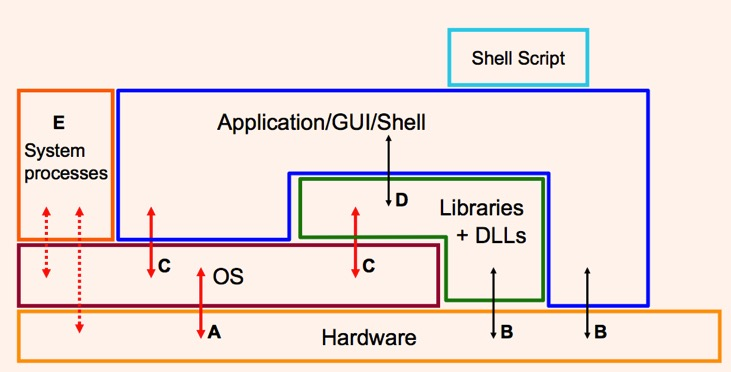
\includegraphics[scale=0.3]{m1/operatingSystemStructure}
		\centering
	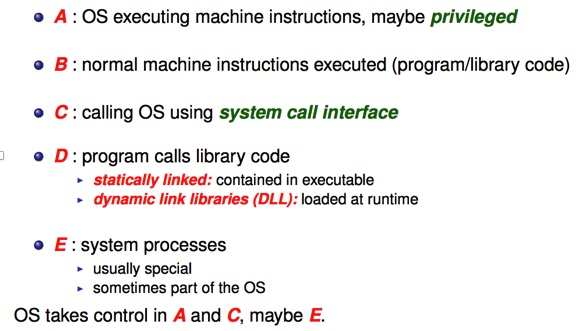
\includegraphics[scale=0.4]{m1/abstractionLayerDescription}
		\centering
\end{tcolorbox}

\begin{definition}{\textbf{Boostrapping}}
	\begin{myitemize}
	\item The \textbf{OS is not present in memory} when a system is “cold started”.
	\begin{myitemize}
		\item When a system is first started up, memory is completely empty.
	\end{myitemize}
	\item We start first with a \textbf{bootloader} to get an operating system into memory.
	\begin{myitemize}
	\item Tiny program in the first (few) sector(s) of the hard-disk.
	\item The first sector is generally called the “boot sector” or “master boot record” for this reason.
	\item Job is to load up the main part of the operating system and start it up.
	\end{myitemize}
\end{myitemize}
\end{definition}

\begin{definition}{\textbf{Core}}
	CPU units that can execute processes, because we have much more number of processes than the number of cores, we have to do \textbf{context switching} to share a core very quickly between different processes.
	\begin{myitemize}
		\item Entire sharing must be transparent.
		\item Processes can be suspended and resumed arbitrarily.
	\end{myitemize}
\end{definition}

\begin{definition}{\textbf{Context switching}}
	\begin{myenumerate}
		\item Save the \textsf{context} of the process to be suspended.
		\item Restore the \textsf{context} of the process to be (re)started.
		\item Issues of \textsf{scheduling} to decide which process to run.
	\end{myenumerate}
\end{definition}

\begin{definition}{\textbf{File system}}
	A set of data structures on disk and within the OS kernel memory to organise persistent data.
\end{definition}

\begin{tcolorbox}
\textsf{How OS file system works?}

	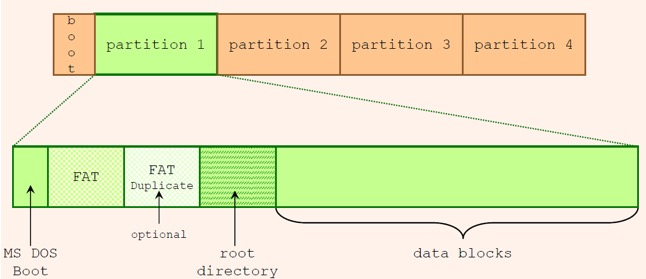
\includegraphics[scale=0.3]{m1/fileSystem}
	\centering
\end{tcolorbox}

\begin{tcolorbox}
	\textsf{Hardware Interfaces}
	
	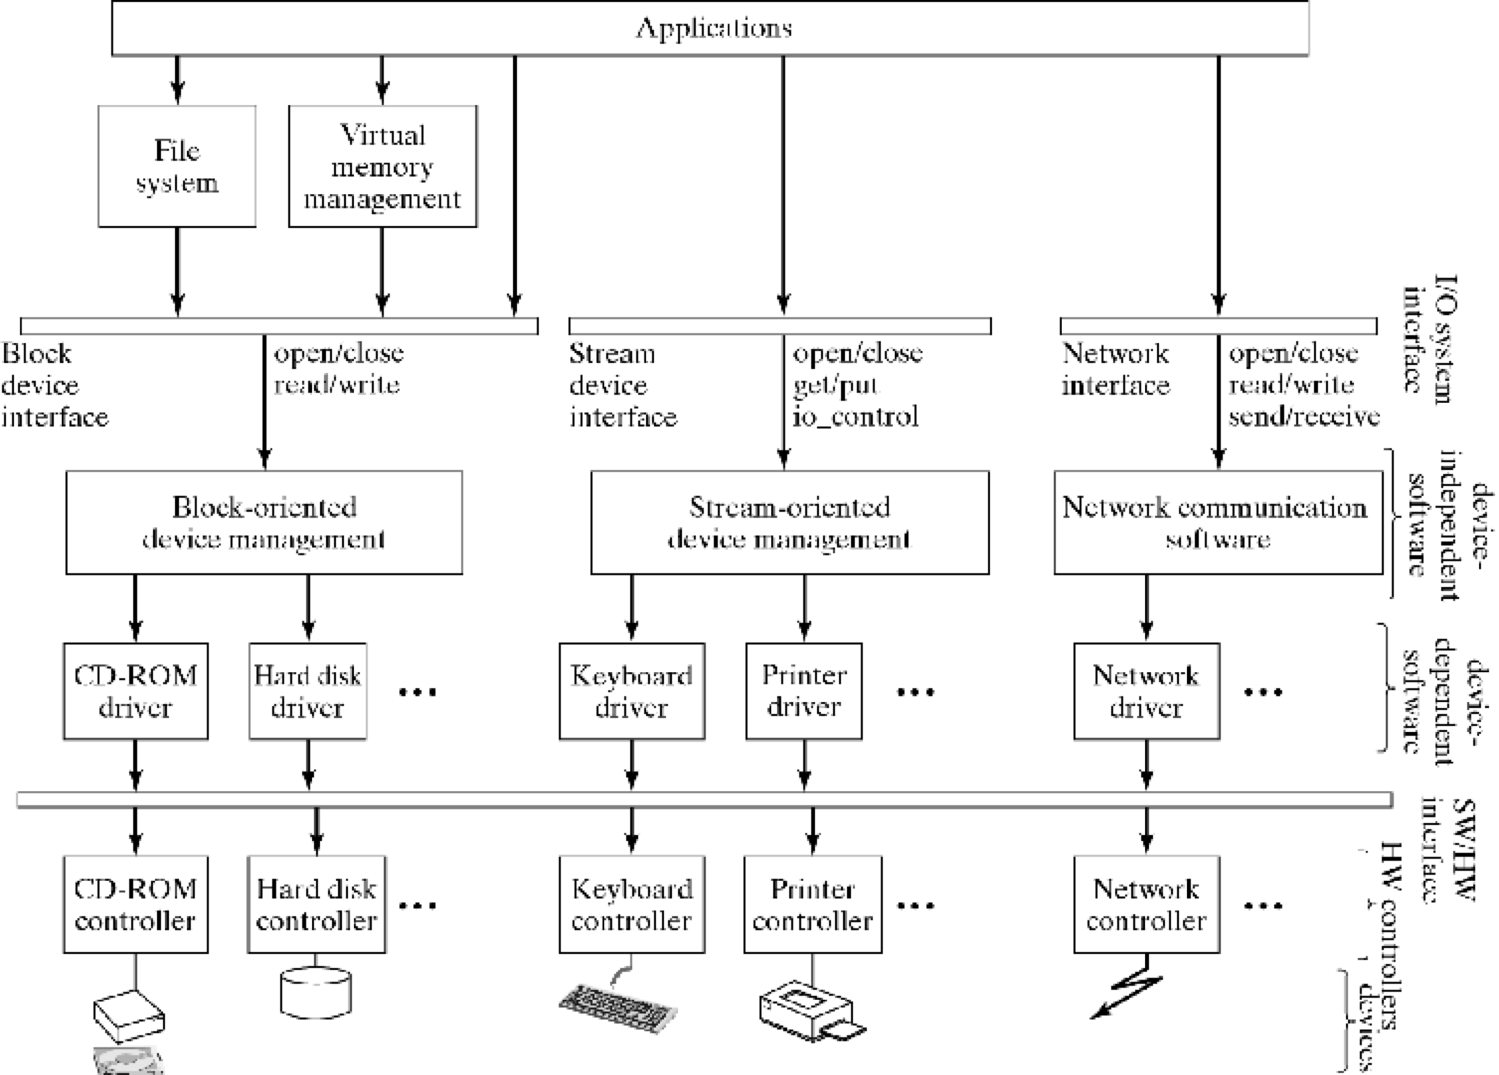
\includegraphics[scale=0.3]{m1/hardwareDevice}
	\centering
	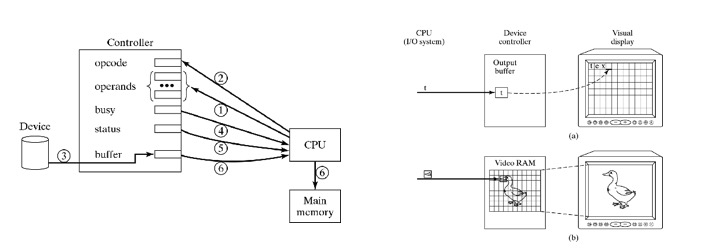
\includegraphics[scale=0.4]{m1/hardwareController}
	\centering
\end{tcolorbox}

\begin{definition}{\textbf{Memory}}
	static/dynamic (\textsf{new, delete, malloc, free}). Memory to store instructions
Memory to store data.
\end{definition}

\begin{tcolorbox}
	\textsf{Memory Management}
	
	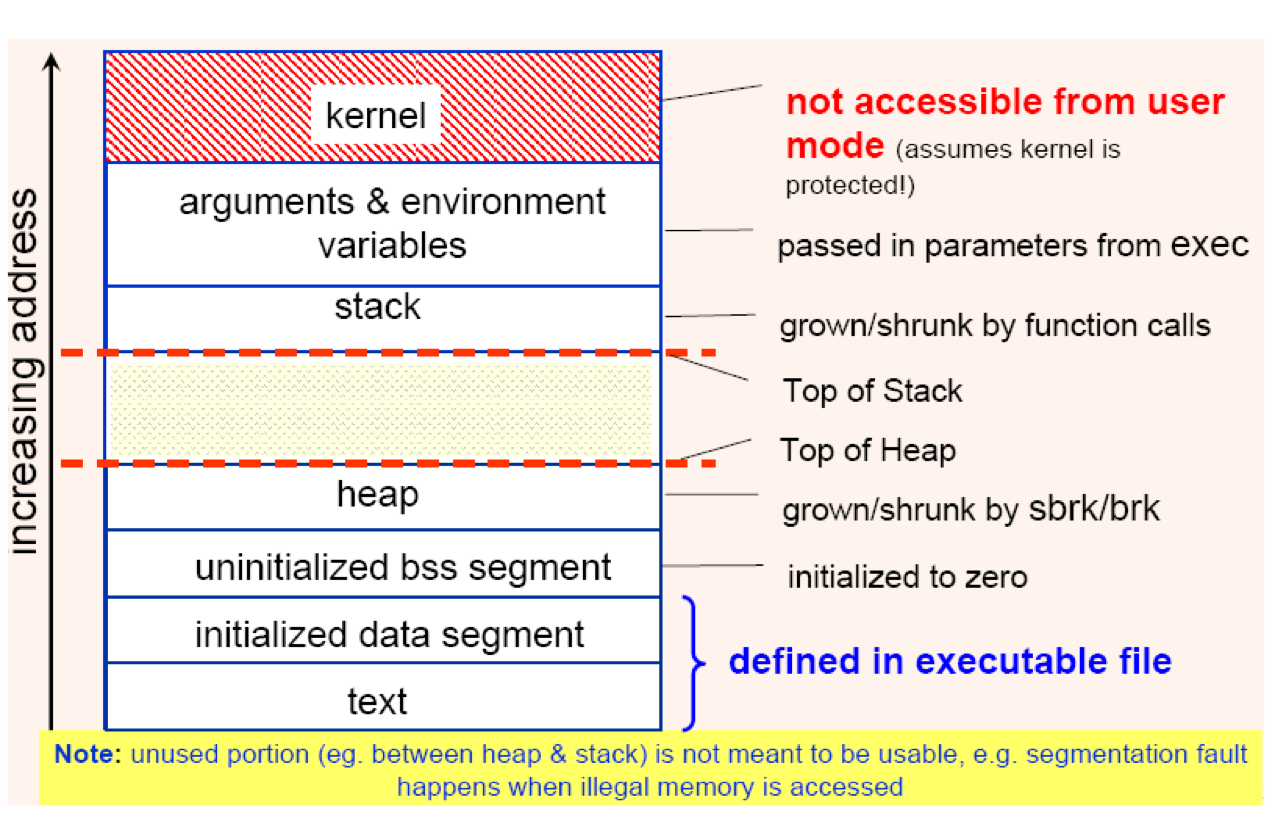
\includegraphics[scale=0.3]{m1/memoryManagement}
	\centering
\end{tcolorbox}

\begin{definition}{\textbf{Virtual Memory management}}
\begin{myitemize}
	\item For cost/speed reasons memory is organized in a hierarchy:
	\begin{figure}[h!]
		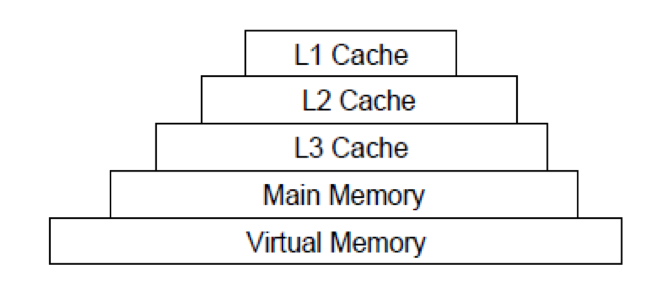
\includegraphics[scale=0.6]{m1/memoryHirarchy}
		\centering
	\end{figure}
	\item The lowest level is called ''virtual memory'' and is the slowest but cheapest memory.
	\begin{myitemize}
	\item Actually made using hard-disk space!
	\item Allows us to fit much more instructions and data than memory allows!
	\end{myitemize}
\end{myitemize}
\end{definition}

\begin{definition}{\textbf{OS security}}
	\begin{myitemize}
		\item Data (files): Encryption techniques, Access control lists
		\item Resources: Access to the hardware (biometric, passwords, etc), Memory access, File access, etc.
	\end{myitemize}
\end{definition}

\begin{tcolorbox}
	\textsf{Writing an OS (BSD Unix)}
	
	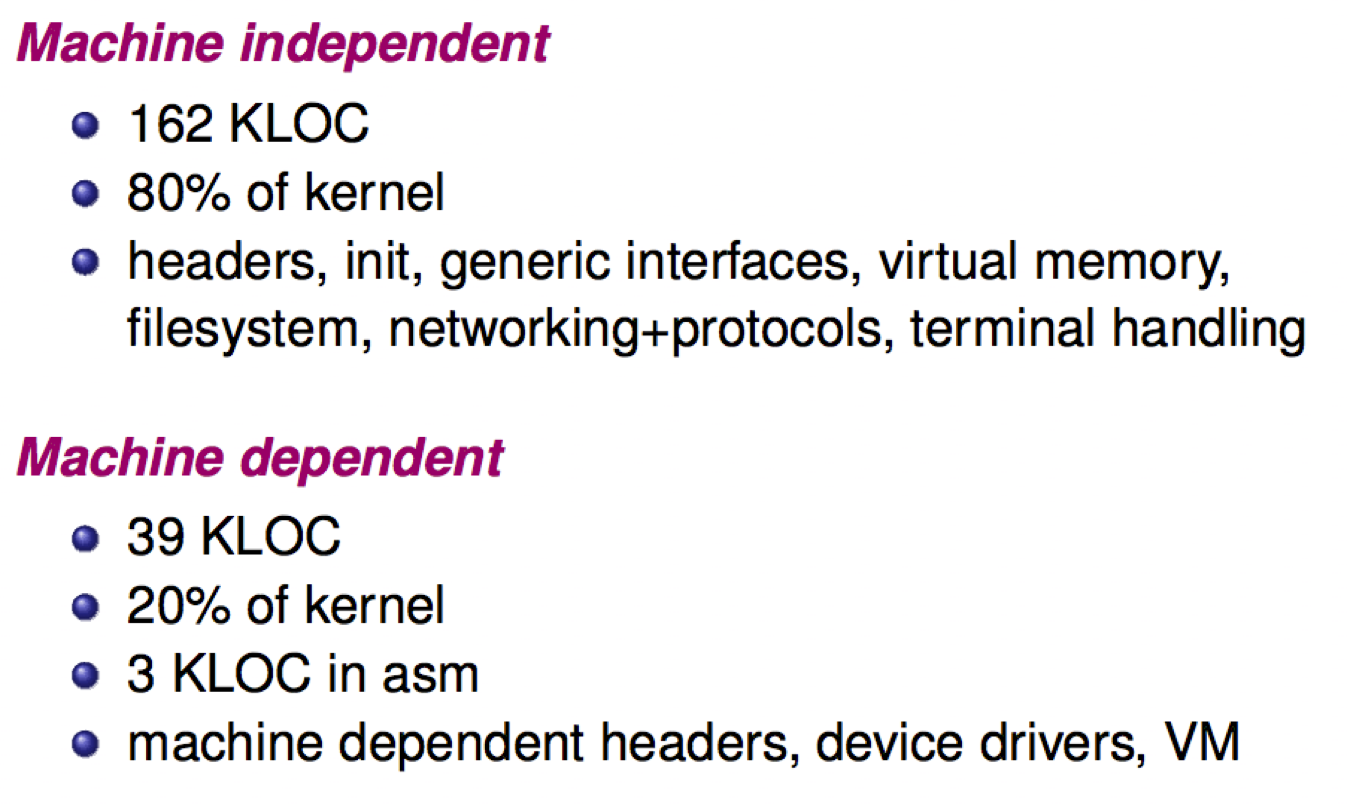
\includegraphics[scale=0.3]{m1/writingOS}
	\centering
\end{tcolorbox}

\begin{definition}{\textbf{Kernel}}
	\begin{myitemize}
		\item \textsf{Monolithic Kernel} (Linux, MS Windows)
		\begin{myitemize}
			\item All major parts of the OS-devices drivers, file systems, IPC, etc, running in ''kernel space'' (an elevated execution mode where certain privileged operations are allowed).
			\item Bits and pieces of the kernel can be loaded and unloaded at runtime (e.g. using ''modprobe'' in Linux)
			\begin{figure}[h!]
				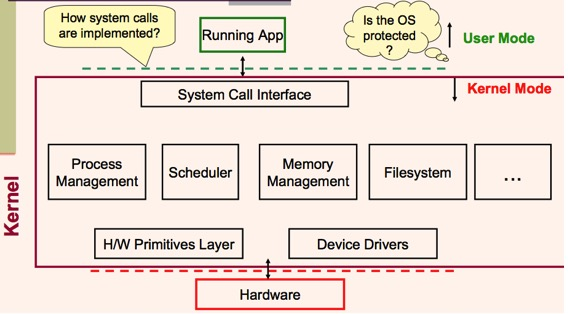
\includegraphics[scale=0.35]{m1/monolithicKernels}
				\centering
			\end{figure}
		\end{myitemize}
		\item \textsf{MicroKernel} (Mac OS)
		\begin{myitemize}
			\item Only the ''main'' part of the kernel is in ''kernel space'' (Contains the important stuff like the scheduler, process management, memory management, etc.)
			\item The other parts of the kernel operate in ''user space'' as system services: The file systems, USB device drivers, Other device drivers.
		\end{myitemize}
	\end{myitemize}
\end{definition}

\begin{tcolorbox}
	\textsf{External View of an OS}
	\begin{myitemize}
		\item The kernel itself is not very useful. (Provides key functionality, but need a way to access all this functionality.)
		\item We need other components:
		\begin{myitemize}
			\item System libraries (e.g. stdio, unistd, etc.)
			\item System services (creat, read, write, ioctl, sbrk, etc.)
			\item OS Configuration (task manager, setup, etc.)
			\item System programs (Xcode, vim, etc.)
			\item Shells (bash, X-Win, Windows GUI, etc.)
			\item Admin tools (User management, disk optimization, etc.)
			\item User applications (Word, Chrome, etc).
		\end{myitemize}
	\end{myitemize}
	
\end{tcolorbox}

\begin{definition}{\textbf{System Calls}}
	calls made to the “Application Program Interface” or API of the OS.
	\begin{myitemize}
		\item UNIX  and similar OS mostly follow the POSIX standard. (Based on C. Programs become more portable.) \textit{POSIX: portable operating system interface for UNIX, minimal set of system calls for application portability between variants of UNIX}.
		\item Windows follows the WinAPI standard. (Windows 7 and earlier provide Win32/Win64, based on C.
Windows 8 provide Win32/Win64 (based on C) and WinRT (based on C++).)
	\end{myitemize}
\end{definition}

\begin{example}{\textbf{User mode + Kernel mode}}
	\begin{myitemize}
		\item Programs (process) run in user mode.
		\item During system calls, running kernel code in kernel mode.
		\item After system call, back to user mode.
	\end{myitemize}
\end{example}

\begin{tcolorbox}
	\textsf{How to switch mode?} Use privilege mode to switching instructions:
	\begin{myitemize}
		\item syscall instruction
		\item software interrupt - instruction which raises specific interrupt from software.
	\end{myitemize}
\end{tcolorbox}

\begin{example}{\textbf{LINUX system call}}
	\begin{myitemize}
		\item User mode: (outside kernel)
		\begin{myitemize}
			\item C function wrapper (eg. \textbf{getpid()}) for every system call in C library.
			\item assembler code to setup the system call no, arguments
			\item trap to kernel	
		\end{myitemize}
		\item Kernel mode: (inside kernel)
		\begin{myitemize}
			\item dispatch to correct routine
			\item check arguments for errors (eg. invalid argument, invalid address, security violation)
			\item do requested service
			\item return from kernel trap to user mode
		\end{myitemize}
		\item User mode: (Outside kernel)
		\begin{myitemize}
			\item returns to C wrapper - check for error return values
		\end{myitemize}
	\end{myitemize}
\end{example}



\section{Process Management}
\begin{definition}{\textbf{Program}}
	consists of: Machine instructions (and possibly source code) and Data. A program exists as a file on the disk. (e.g. command.exe, MSword.exe)
\end{definition}

\begin{definition}{\textbf{Process}}
	consists of Machine instructions (and possibly source code), Data and Context. It exists as instructions and data in memory, \textbf{may} be executing on the CPU.
\end{definition}

\begin{tcolorbox}
	\textsf{Program vs. Process}
	
	A single program can produce multiple processes. (e.g. chrome.exe is a single program, but every tab in Chrome is a new process!)

\end{tcolorbox}

\begin{definition}{\textbf{Execution Modes}}
	\begin{myitemize}
		\item Programs usually run sequentially. (Each instruction is executed one after the other.)
		\item Having multiple cores or CPUs allow parallel (''concurrent'') execution. (Streams of instructions with no dependencies are allowed to execute together.)
		\item A multitasking OS allows several programs to run ''concurrently''. (Interleaving, or “time-slicing”)
	\end{myitemize}
\end{definition}

\begin{remark}
	we mostly assume number of processes $\geq$ number of CPU otherwise can have idle tasks. So each core must still switch between processes even for multi-cores, and we will assume a single processor with a single core.
\end{remark}

\begin{tcolorbox}
	\textsf{The Process Model}
	
	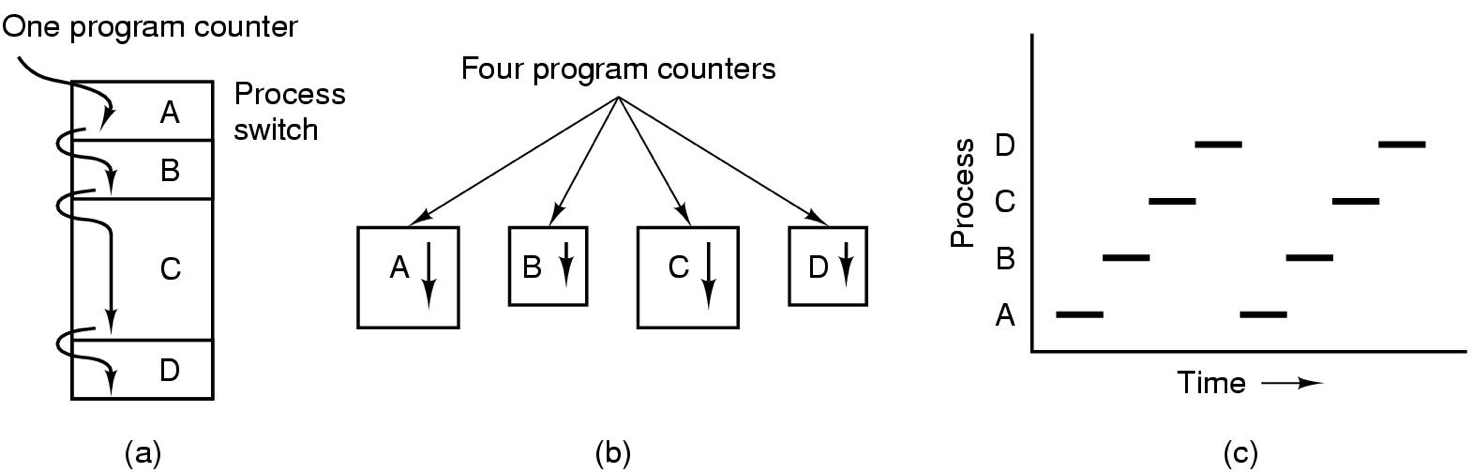
\includegraphics[scale=0.5]{m1/processModel}
	\centering
	
	\begin{myitemize}
		\item Figure (b) shows what “appears” to be happening in a single processor system running multiple processes:
		\begin{myitemize}
			\item There are 4 processes each with its own program counter (PC) and registers.
			\item All 4 processes run independently of each other at the same time.
		\end{myitemize}
		\item Figure (a) shows what actually happens.
		\begin{myitemize}
			\item There is only a single PC and a single set of registers.
			\item When one process ends, there is a ''context switch'' or ''process switch'':
			\begin{myitemize}
				\item PC, all registers and other process data for Process A is copied to memory.
				\item PC, register and process data for Process B is loaded and B starts executing, etc.
			\end{myitemize}
		\end{myitemize}
		\item Figure (c) illustrates how processes A to D share CPU time.
	\end{myitemize}
\end{tcolorbox}

\begin{definition}{\textbf{Process States}} there are three possible states for a process
	\begin{myitemize}
		\item Running 
		\begin{myitemize}
			\item The process is actually being executed on the CPU.
		\end{myitemize}
		\item Ready 
		\begin{myitemize}
			\item The process is ready to run but not currently running. 
			\item A ''scheduling algorithm'' is used to pick the next process for running.
		\end{myitemize}
		\item Blocked.
		\begin{myitemize}
			\item The process is waiting for ''something'' to happen so it is not ready to run yet. e.g. include waiting for inputs from another process.
		\end{myitemize}
	\end{myitemize}
\end{definition}

\begin{figure}[h!]
	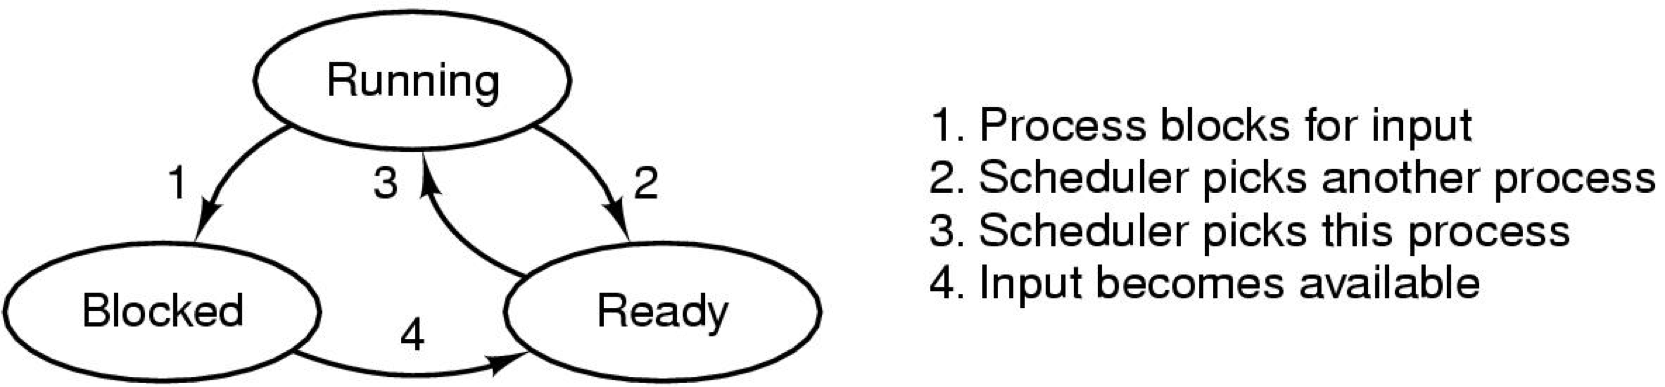
\includegraphics[scale=0.3]{m1/processStates}
	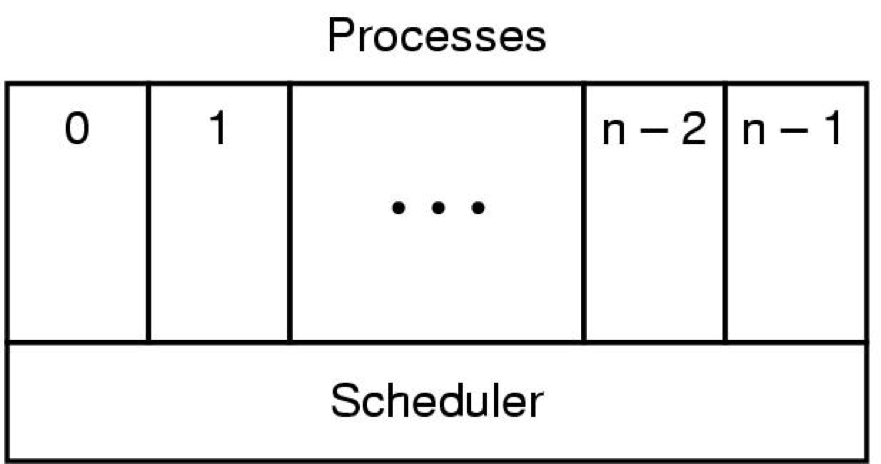
\includegraphics[scale=0.3]{m1/processStates2}
	\centering
\end{figure}

\begin{definition}{\textbf{Process Context}} (values change as a process runs)
	\begin{myitemize}
		\item CPU register values. 
		\item Stack pointers.
		\item CPU Status Word Register
		\begin{myitemize}
			\item This maintains information about whether the previous instruction resulted in an overflow or a ''zero'', whether interrupts are enabled, etc.
			\item This is needed for branch instructions – assembly equivalents of ''if'' statements.
		\end{myitemize}
	\end{myitemize}
\end{definition}

\begin{figure}[h!]
	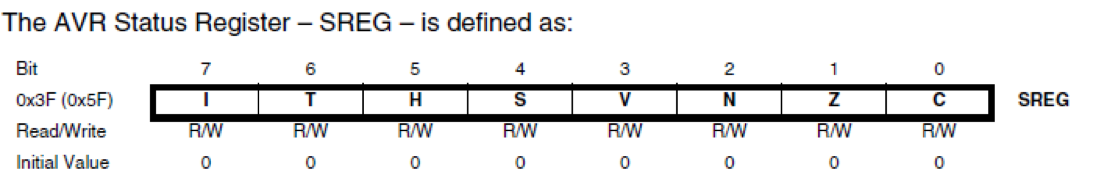
\includegraphics[scale=0.6]{m1/statusRegister}
	\centering
\end{figure}

\begin{example}{\textbf{Context Switching in FreeRTOS Atmega Port}}
	FreeRTOS relies on regular interrupts from Timer 0 to switch between tasks. When the interrupt triggers:
	\begin{myenumerate}
		\item PC is placed onto Task A’s stack.
		\item The ISR calls \textsf{portSAVECONTEXT}, resulting in Task A’s context being pushed onto the stack. 
		\item \textsf{pxCurrentTCB} will also hold SPH/SPL after the context save.
		\begin{myitemize}
			\item This must be saved by the kernel.
			\item The kernel stores a copy of the stack pointer for each task.
		\end{myitemize}
		\item The kernel then selects Task B to run, and copies its SPH/SPL values into \textsf{pxCurrentTCB} and calls \textsf{portRESTORE\_CONTEXT}.
		\item The rest of \textsf{portRESTORE\_CONTEXT} is executed, causing Task B’s data to be loaded into R31-R0 and SREG. Now Task B can resume like as though nothing happened
		\item Only Task B’s PC remains on the stack. Now the ISR exits, causing this value to be popped off onto the AVR’s PC.
		\begin{myitemize}
			\item PC points to the next instruction to be executed. 
			\item End result: Task B resumes execution, with all its data and SREG intact!
		\end{myitemize}
	\end{myenumerate}
\end{example}

\begin{tcolorbox}
	\textsf{How can context switching be triggered?}
	
	It can be triggered by a timer; currently running process waiting for input; currently running task blocking on a synchronisation mechanism; currently running task wants to sleep for a fixed period; higher priority task becoming “READY”; $\dots$
\end{tcolorbox}

\begin{definition}{\textbf{Process Control Block}}
	maintains information about that process: Process ID (PID), Stack Pointer, Open files, Pending signals, CPU usage, $\dots$
\end{definition}

\begin{tcolorbox}
	\textsf{Process Life Cycle}
	
	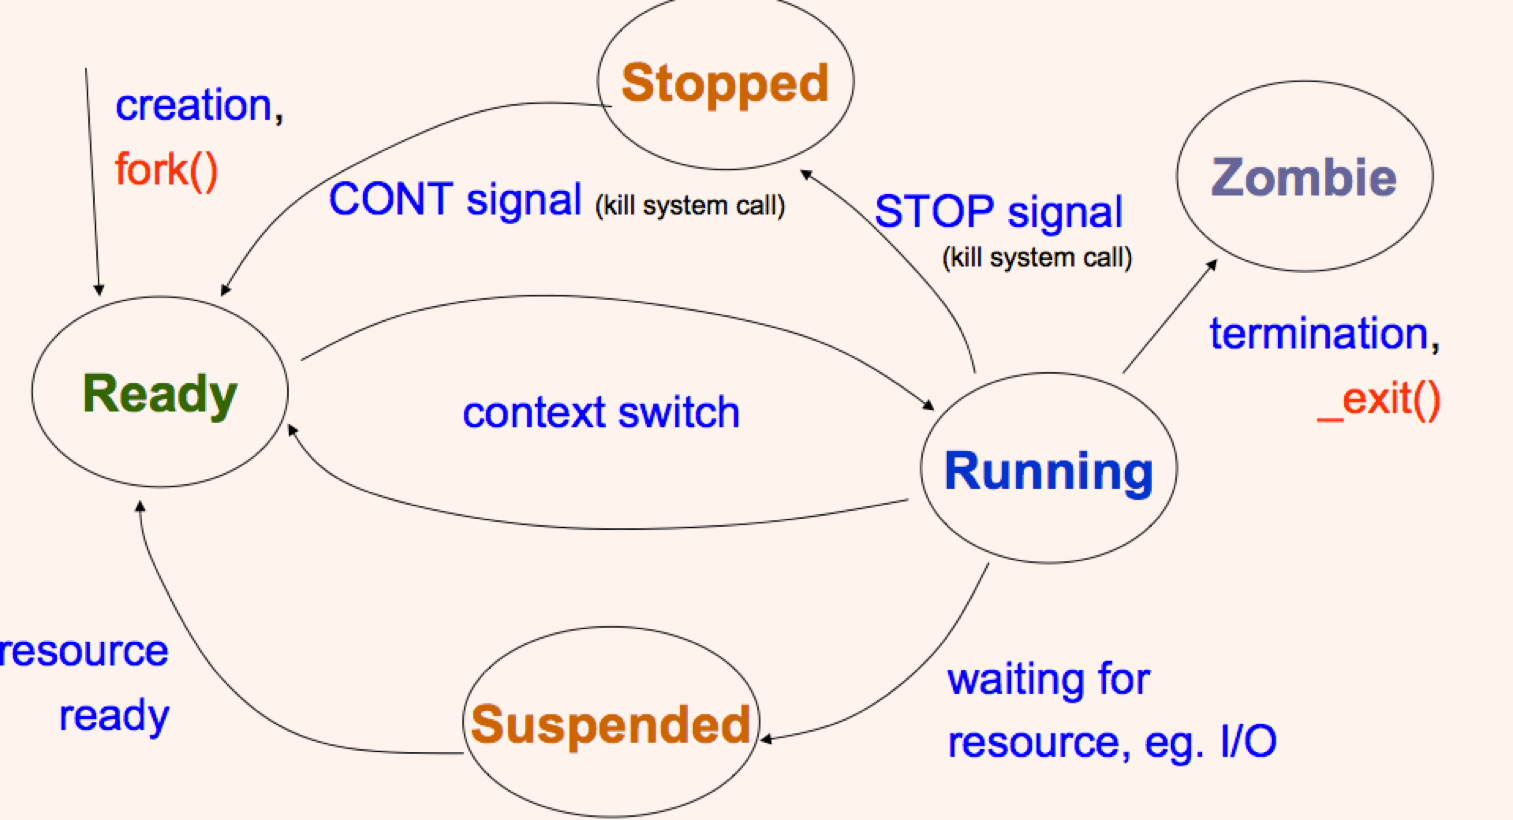
\includegraphics[scale=0.3]{m1/processLifeCycle}
	\centering
\end{tcolorbox}

\begin{definition}{\textbf{Creating a new process - fork()}}
	\begin{myitemize}
		\item Fork system call creates a new process by duplicating the current image into a new process, \textit{child process}
		\item \textsf{same code} (executable image) is executed
		\item Child differs only in process id (PID) and parent (PPID), fork return value
		\item Data in child is a COPY of the parent (i.e. not shared)
		\item In PARENT process after fork:
		\begin{myitemize}
			\item PC is at return from fork system call
			\item fork return value: new child PID
		\end{myitemize}
		\item In CHILD process after fork:
		\begin{myitemize}
			\item PC is at return from fork system call
			\item fork return value: 0
			\item Shares open file \& signal handlers with parent, current working directory
			\item Independent copy of: memory, arguments, environment variables (note: cloning example)
		\end{myitemize}
		\item fork return result is -1 if the fork failed.
	\end{myitemize}
\end{definition}

\begin{definition}{\textbf{The Master Process}}
	\begin{myitemize}
		\item Every process has parent: \textsf{where does it stop?}
		\item Special initial process - \textsf{init} process created in kernel at the end UNIX boot process, traditionally having PID=1.
		\item Forking creates process tree, \textsf{init} is the root process.
		\item \textsf{init} watches for processes and response where needed, e.g. terminal login.
		\item \textsf{init} also manages system run levels (e.g. shutdown, power failure, single-user mode), etc. Example of a system-like process running in kernel mode.
	\end{myitemize}
\end{definition}

\begin{definition}{\textbf{Start/Stop a Process}}
	\begin{myitemize}
		\item kill() system call sends signal to process
		\item Special process signals:
		\begin{myitemize}
			\item stopping process (SIGSTOP)
			\item killing process (SIGKILL)
			\item restart stopped process (SIGCONT)
		\end{myitemize}
	\end{myitemize}
\end{definition}

\begin{tcolorbox}
	\textsf{Terminating a process}
	
	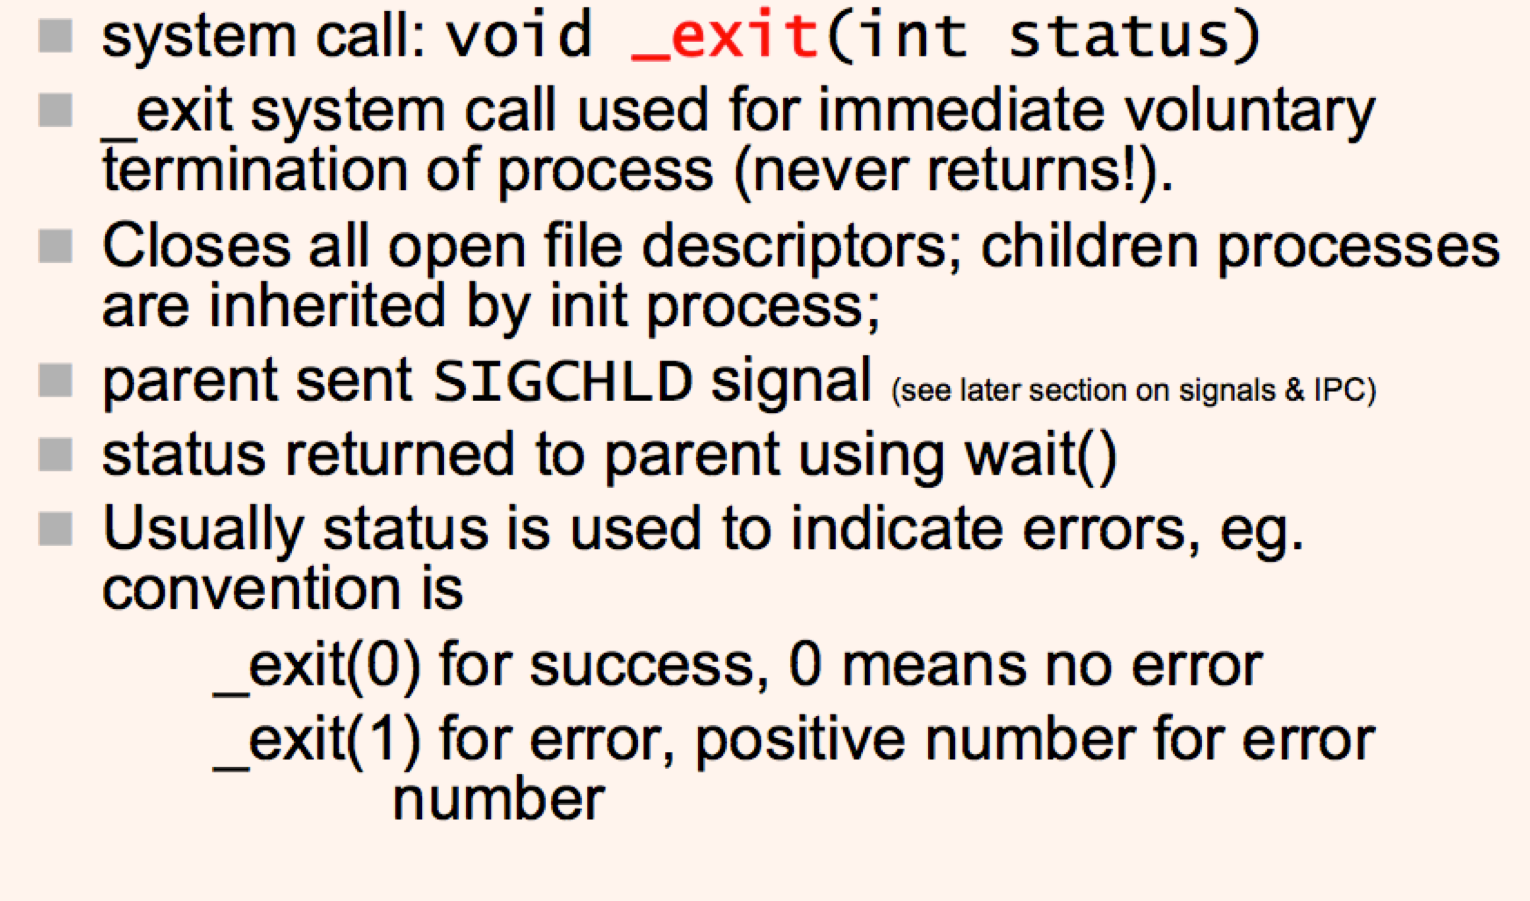
\includegraphics[scale=0.33]{m1/terminatingProcess1}
	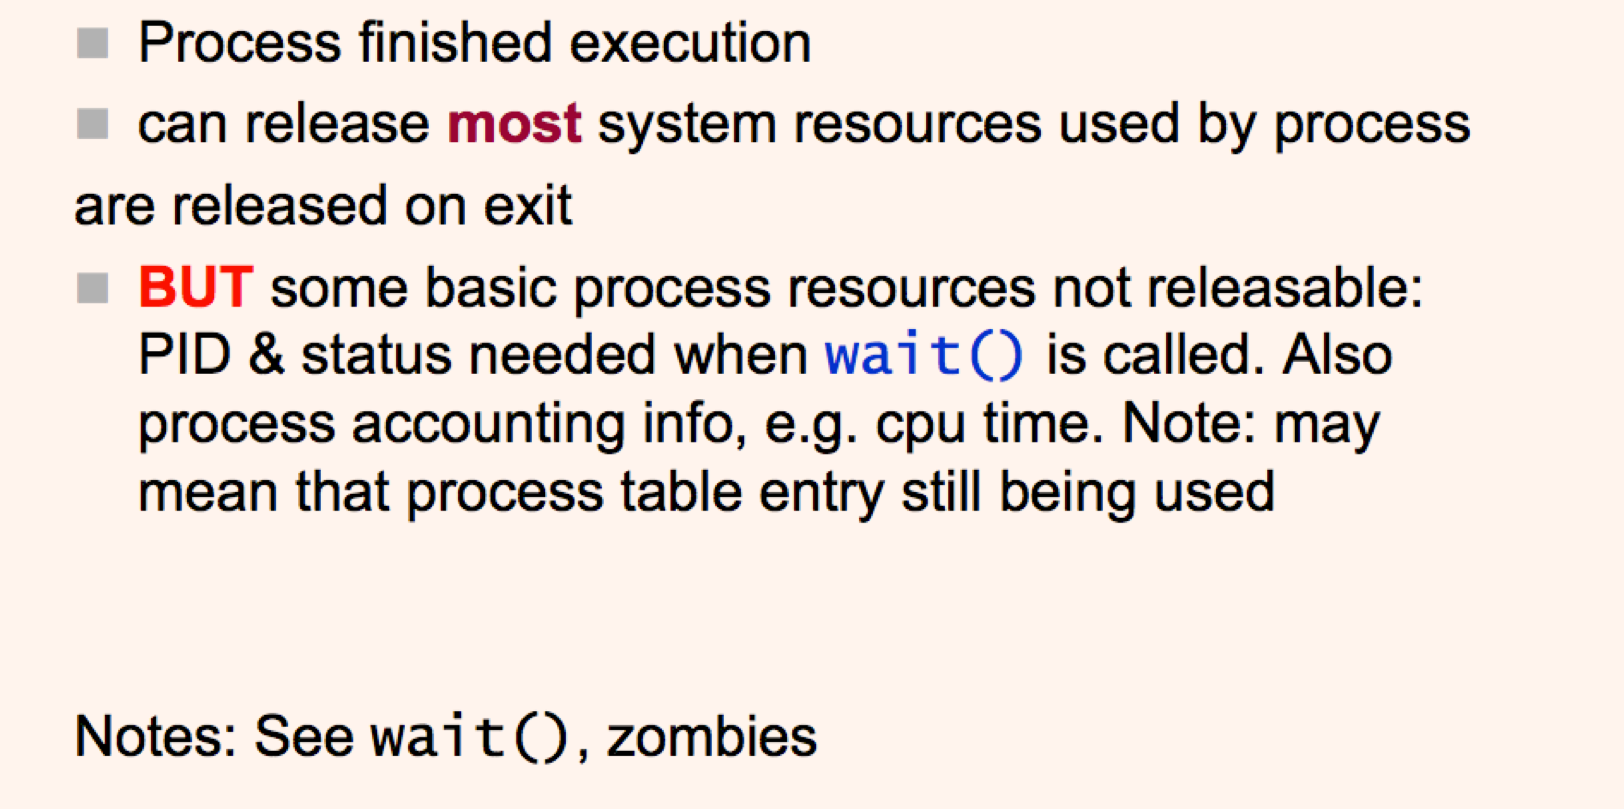
\includegraphics[scale=0.33]{m1/terminatingProcess2}
	\centering
\end{tcolorbox}

\begin{definition}{\textbf{Normal Program Termination} - \textsf{void exit(int status)} from standard C library function}
	\begin{myitemize}
		\item Usuall don't use \textsf{\_exit()} but \textsf{exit()}, which cleans up: open streams from C stdio library (e.g., fopen, printf) are flushed and closed
		\item calls some exit handlers
		\item finally calls \textsf{\_exit(status)} after all standard C cleanup done.
	\end{myitemize}
\end{definition}
\begin{remark}
	returning from \textsf{main()} implicitly calls exit. \textsf{exec} didn't actually call main directly but a startup routine. Open files also get flushed automatically.
\end{remark}

\begin{tcolorbox}
	\textsf{Waiting for Child Processes to Terminate - process interaction}
	
	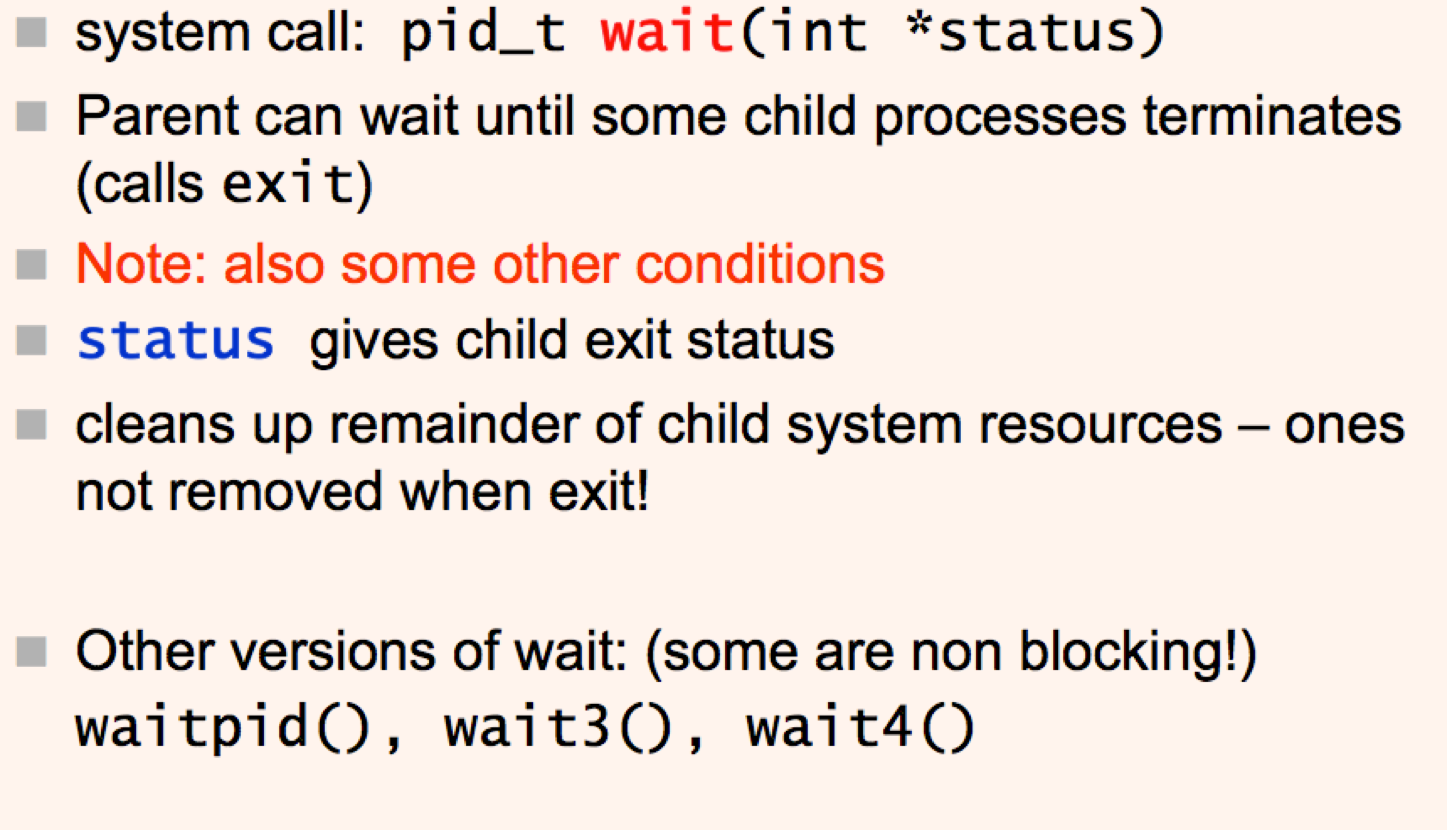
\includegraphics[scale=0.33]{m1/parentWait1}
	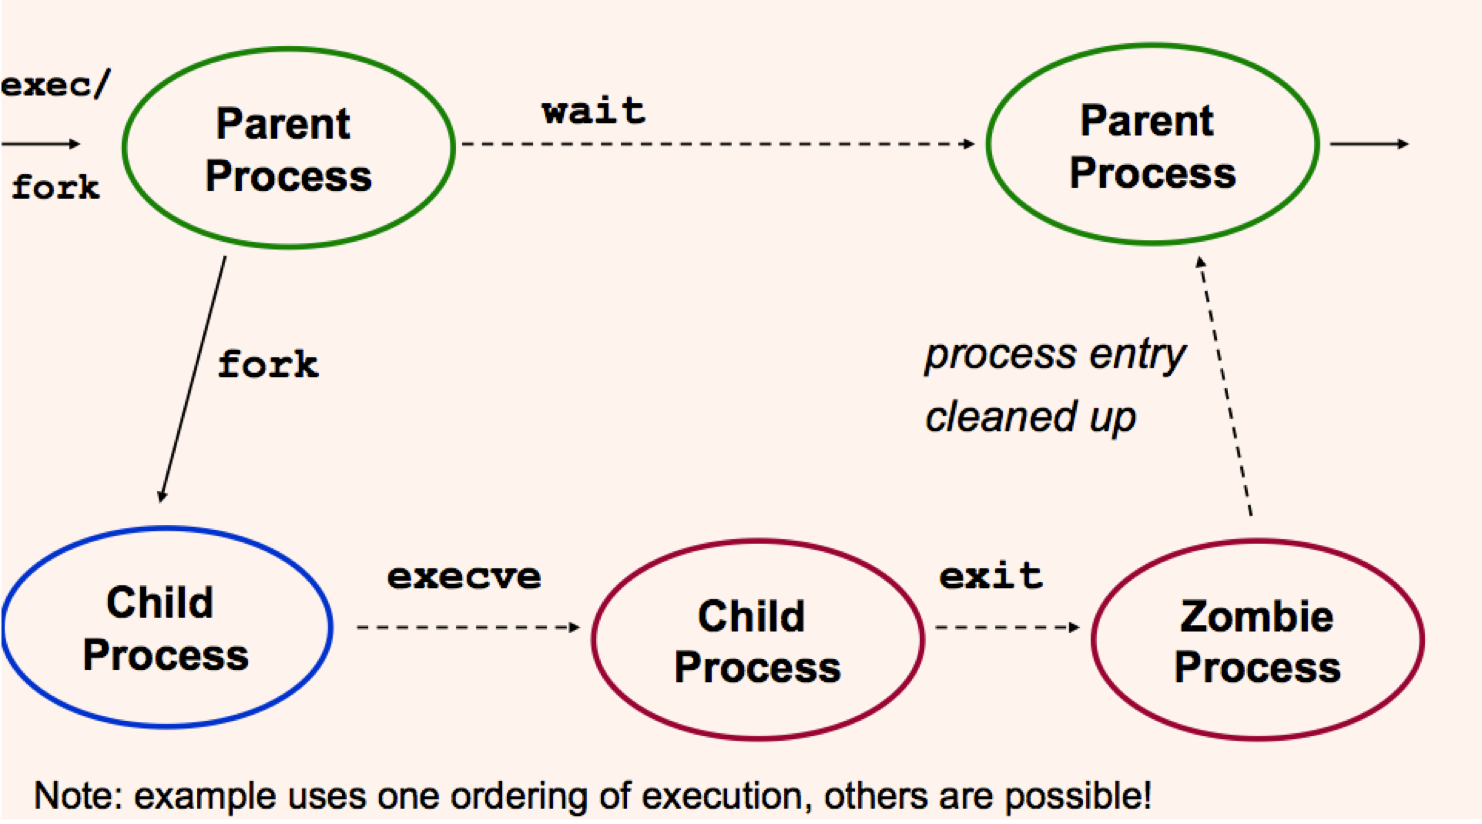
\includegraphics[scale=0.33]{m1/parentWait2}
	\centering
\end{tcolorbox}

\begin{tcolorbox}
	\textsf{Zombie Process}
	
	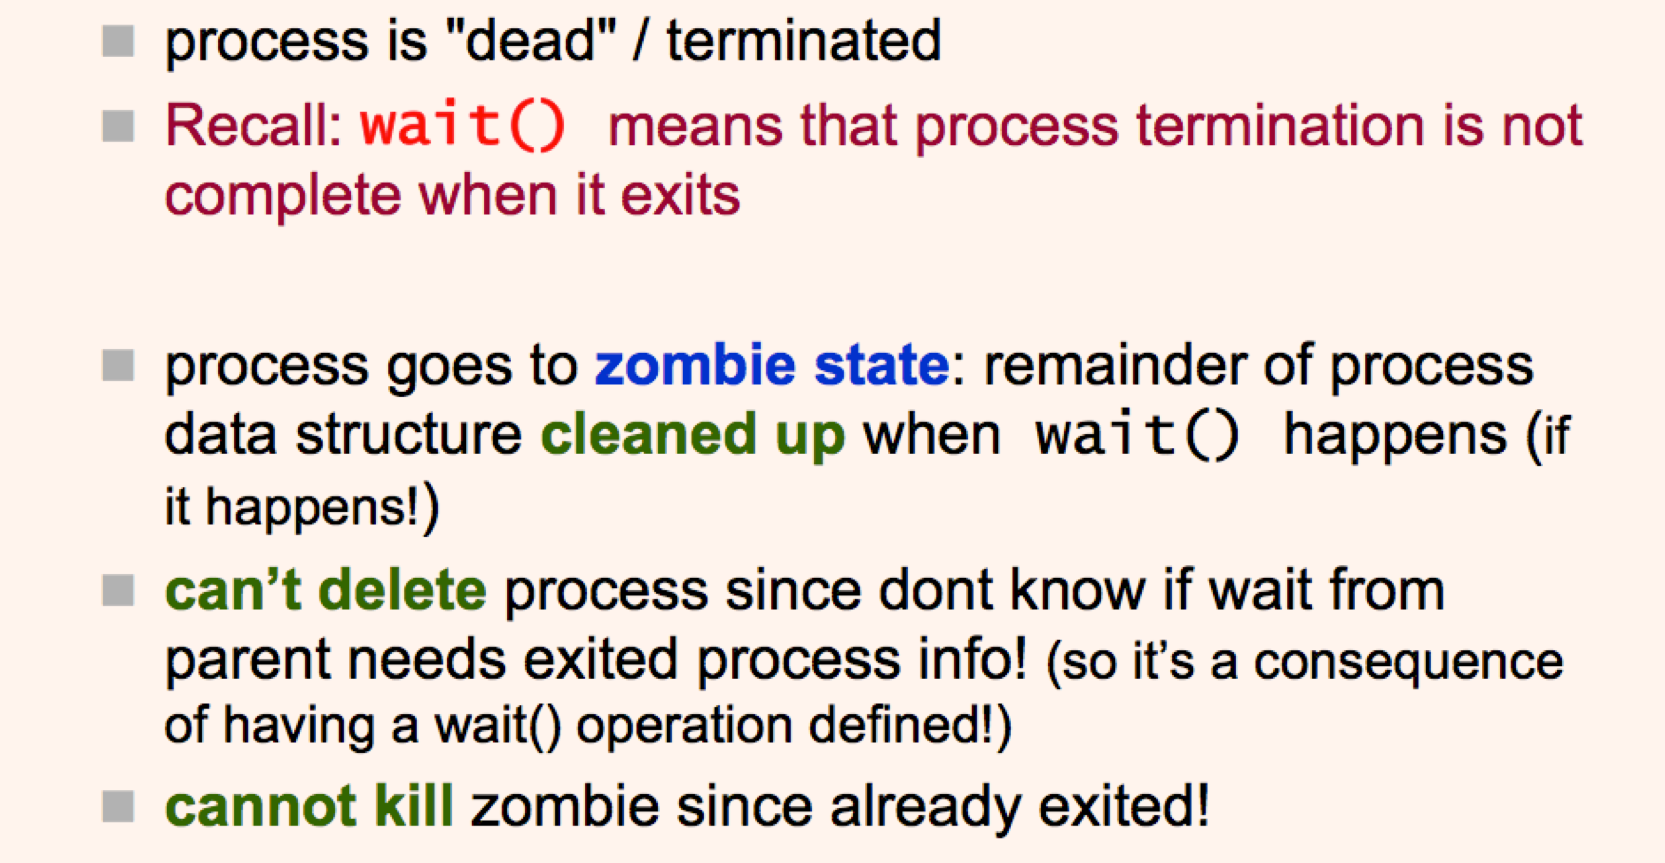
\includegraphics[scale=0.30]{m1/zombieProcess1}
	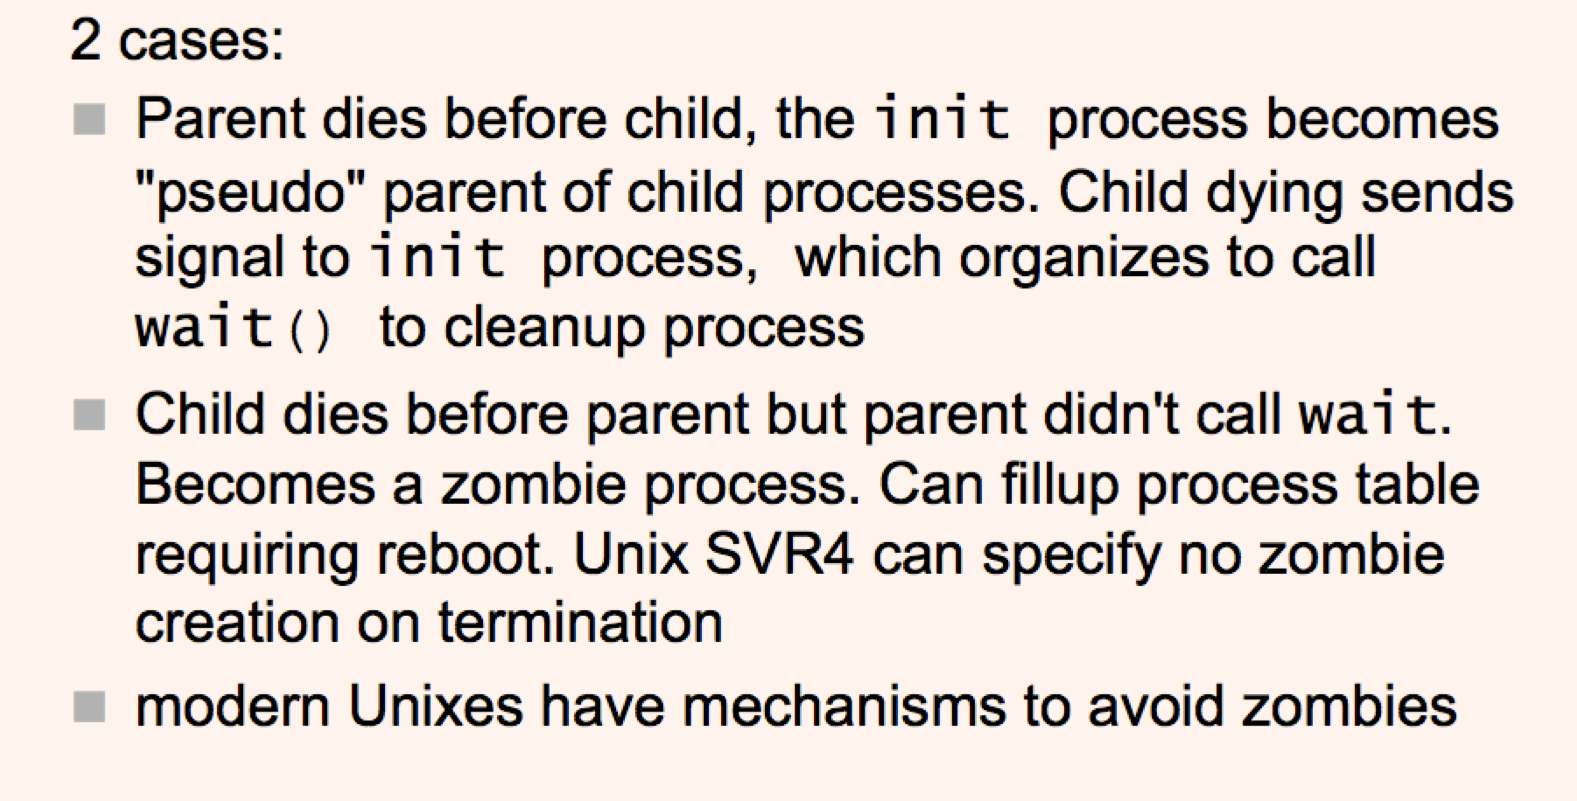
\includegraphics[scale=0.30]{m1/zombieProcess2}
	\centering
\end{tcolorbox}

\section{Process Scheduling}





















% $$$$$$$$$$$$$$$$$$$$$$$$$$$$$$$$$$ %

\end{document}